\begin{tikzpicture} 
\begin{axis}[
axis lines*=middle,
enlargelimits = true,
ymin=-1.2,
ymax=1.2,
xmin=0,
xmax=10,
axis line style={->,>=stealth},
%xlabel={\Large $n$},
%ylabel={\Large $x[n]$},
yticklabel style = {yshift=0.2cm},
xticklabel style = {yshift=-0.1cm},
every axis x label/.style={
    at={(ticklabel* cs:1)},
    anchor=north,
},
every axis y label/.style={
    at={(ticklabel* cs:1)},
    anchor=south,
},
%xtick=\empty,
ytick=\empty,
xtick=\empty,
every outer y axis line/.append style={white!15!black},
every y tick label/.append style={font=\color{white!15!black}},
legend style={draw=white!15!black,fill=white,legend cell align=left}]

\only<1-|handout:1>{
\addplot[black!50, smooth, line width=1.5pt, domain=0:10, samples=21] {cos(deg(2*pi*0.15*x))};
\addplot[ycomb, mark=*, fill=white, mark options={scale=1, fill=white}, line width=1.5pt, domain=0:10, samples=11] {cos(deg(2*pi*0.15*x))};
}
\only<2|handout:0>{
\foreach \n in {0, 1, ..., 10}
{
	\addplot[red, line width=1pt, domain=\n-1:\n+1, samples=3] {cos(deg(2*pi*0.15*x))*(x == \n)};
}
}
\only<3|handout:1>{
	\foreach \n in {0, 1, ..., 10}
	{
		\addplot[red!30, line width=1pt, domain=\n-1:\n+1, samples=3] {cos(deg(2*pi*0.15*x))*(x == \n)};
	}
	\addplot [color=red, solid, line width=1.5pt, forget plot]
	table[row sep=crcr]{
		0 1 \\
		0.2 0.91756 \\
		0.4 0.83511 \\
		0.6 0.75267 \\
		0.8 0.67023 \\
		1 0.58779 \\
		1.2 0.40842 \\
		1.4 0.22906 \\
		1.6 0.049704 \\
		1.8 -0.12966 \\
		2 -0.30902 \\
		2.2 -0.43742 \\
		2.4 -0.56583 \\
		2.6 -0.69424 \\
		2.8 -0.82265 \\
		3 -0.95106 \\
		3.2 -0.92265 \\
		3.4 -0.89424 \\
		3.6 -0.86583 \\
		3.8 -0.83742 \\
		4 -0.80902 \\
		4.2 -0.64721 \\
		4.4 -0.48541 \\
		4.6 -0.32361 \\
		4.8 -0.1618 \\
		5 -1.837e-16 \\
		5.2 0.1618 \\
		5.4 0.32361 \\
		5.6 0.48541 \\
		5.8 0.64721 \\
		6 0.80902 \\
		6.2 0.83742 \\
		6.4 0.86583 \\
		6.6 0.89424 \\
		6.8 0.92265 \\
		7 0.95106 \\
		7.2 0.82265 \\
		7.4 0.69424 \\
		7.6 0.56583 \\
		7.8 0.43742 \\
		8 0.30902 \\
		8.2 0.12966 \\
		8.4 -0.049704 \\
		8.6 -0.22906 \\
		8.8 -0.40842 \\
		9 -0.58779 \\
		9.2 -0.67023 \\
		9.4 -0.75267 \\
		9.6 -0.83511 \\
		9.8 -0.91756 \\
		10 -1 \\
		10.2 -0.91756 \\
		10.4 -0.83511 \\
		10.6 -0.75267 \\
		10.8 -0.67023 \\
		11 -0.58779 \\
		11.2 -0.40842 \\
		11.4 -0.22906 \\
		11.6 -0.049704 \\
		11.8 0.12966 \\
		12 0.30902 \\
		12.2 0.43742 \\
		12.4 0.56583 \\
		12.6 0.69424 \\
		12.8 0.82265 \\
		13 0.95106 \\
		13.2 0.92265 \\
		13.4 0.89424 \\
		13.6 0.86583 \\
		13.8 0.83742 \\
		14 0.80902 \\
		14.2 0.64721 \\
		14.4 0.48541 \\
		14.6 0.32361 \\
		14.8 0.1618 \\
		15 5.5109e-16 \\
		15.2 -0.1618 \\
		15.4 -0.32361 \\
		15.6 -0.48541 \\
		15.8 -0.64721 \\
		16 -0.80902 \\
		16.2 -0.83742 \\
		16.4 -0.86583 \\
		16.6 -0.89424 \\
		16.8 -0.92265 \\
		17 -0.95106 \\
		17.2 -0.82265 \\
		17.4 -0.69424 \\
		17.6 -0.56583 \\
		17.8 -0.43742 \\
		18 -0.30902 \\
		18.2 -0.12966 \\
		18.4 0.049704 \\
		18.6 0.22906 \\
		18.8 0.40842 \\
		19 0.58779 \\
		19.2 0.67023 \\
		19.4 0.75267 \\
		19.6 0.83511 \\
		19.8 0.91756 \\
		20 1 \\
		20.2 0.91756 \\
		20.4 0.83511 \\
		20.6 0.75267 \\
		20.8 0.67023 \\
	};
	
}
\end{axis}
\end{tikzpicture}